\chapter{Methodology}
\label{ch:methodology}

This project functions as a pilot study in preparation for a bigger project held at the clinic. It is also an explorative study as it may discover new ways to communicate between patients and the hospital, possibly replacing the current way of informing patients. This allows the clinic to run a small-scale project and see how the application compares to the existing system at an early stage with reduced investment and costs.

The development will focus on iterating over designs and prototypes in a user-centered manner. Using this method, potential users and stakeholders will be able to try out the design throughout various phases of its development. This user testing may consist of focus groups and uncontrolled experiments, and the gained experience can be applied in the next development stage. In our case, the testing will be restricted to the internal group at first, but a designated test group will be created once the design evolves into interactive prototypes.

\section{Evaluation}
\label{sec:evaluation}

The final prototype will be evaluated by a usability test. A group of X users will be invited to test and evaluate the application. The users will be handed an interactive prototype and asked to perform certain use cases. In addition, the users will give their impressions of the system through a semi-structured interview. The project is deemed to be valuable if the users find the application to be more informative and engaging than the current system.

"informing", "ease of use", "trustability" and "fun"

\section{Design process}
\label{sec:designprocess}

Iterative

For hver iterasjon
- Hva er problemstillingen?
- Hvilken tilnærming til løsningen skal prototypen ha?
- Hvordan er det levert?
- Hvordan det er testet/testresultater

- Double Diamond approach: solve the right problem

https://www.designcouncil.org.uk/news-opinion/design-process-what-double-Diamond

Må utforske mye før man fokuserer inn på problemstilling - utforskningen er iterativ

\section{Interaction design}
\label{sec:interactiondesign}

\textcite{preece2015} developed a lifecycle model for interaction design that could prove to be useful for this project. This model is shown in \ref{fig:interactiondesign}

\begin{figure}
    \centering
    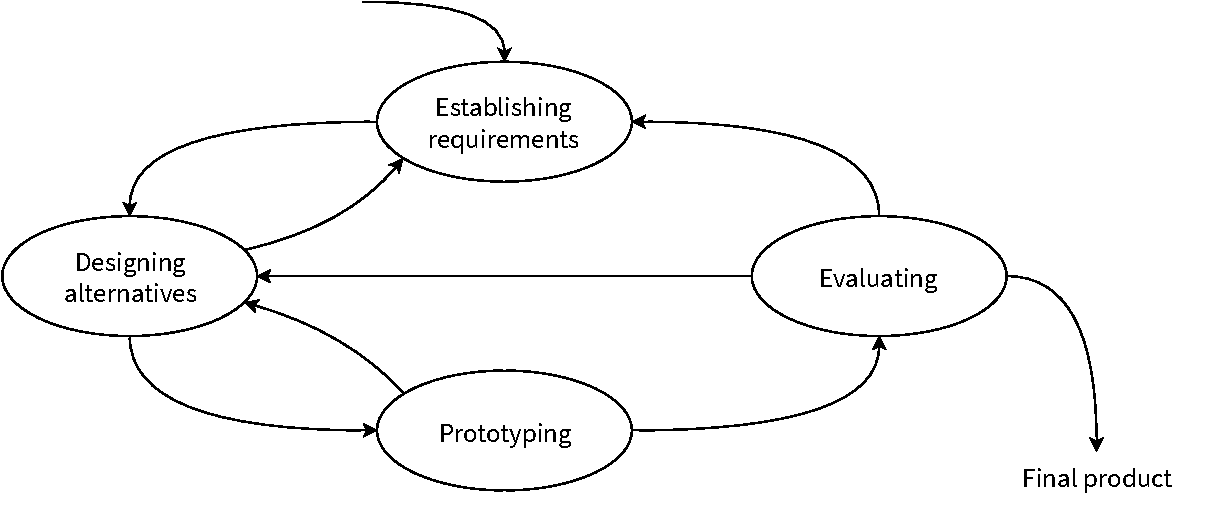
\includegraphics[width=0.75\textwidth]{interaction-design-lifecycle-model.pdf}
    \caption{Interaction design lifecycle model}
    \label{fig:interactiondesign}
\end{figure}

\section{Prototyping}
\label{sec:prototyping}

\subsection{Prototyping tools}

\subsubsection{Pen and paper}

\subsubsection{Online prototyping software}

Marvel

Figma
